\documentclass[]{tufte-handout}

% ams
\usepackage{amssymb,amsmath}

\usepackage{ifxetex,ifluatex}
\usepackage{fixltx2e} % provides \textsubscript
\ifnum 0\ifxetex 1\fi\ifluatex 1\fi=0 % if pdftex
  \usepackage[T1]{fontenc}
  \usepackage[utf8]{inputenc}
\else % if luatex or xelatex
  \makeatletter
  \@ifpackageloaded{fontspec}{}{\usepackage{fontspec}}
  \makeatother
  \defaultfontfeatures{Ligatures=TeX,Scale=MatchLowercase}
  \makeatletter
  \@ifpackageloaded{soul}{
     \renewcommand\allcapsspacing[1]{{\addfontfeature{LetterSpace=15}#1}}
     \renewcommand\smallcapsspacing[1]{{\addfontfeature{LetterSpace=10}#1}}
   }{}
  \makeatother

\fi

% graphix
\usepackage{graphicx}
\setkeys{Gin}{width=\linewidth,totalheight=\textheight,keepaspectratio}

% booktabs
\usepackage{booktabs}

% url
\usepackage{url}

% hyperref
\usepackage{hyperref}

% units.
\usepackage{units}


\setcounter{secnumdepth}{-1}

% citations


% pandoc syntax highlighting
\usepackage{color}
\usepackage{fancyvrb}
\newcommand{\VerbBar}{|}
\newcommand{\VERB}{\Verb[commandchars=\\\{\}]}
\DefineVerbatimEnvironment{Highlighting}{Verbatim}{commandchars=\\\{\}}
% Add ',fontsize=\small' for more characters per line
\newenvironment{Shaded}{}{}
\newcommand{\AlertTok}[1]{\textcolor[rgb]{1.00,0.00,0.00}{\textbf{#1}}}
\newcommand{\AnnotationTok}[1]{\textcolor[rgb]{0.38,0.63,0.69}{\textbf{\textit{#1}}}}
\newcommand{\AttributeTok}[1]{\textcolor[rgb]{0.49,0.56,0.16}{#1}}
\newcommand{\BaseNTok}[1]{\textcolor[rgb]{0.25,0.63,0.44}{#1}}
\newcommand{\BuiltInTok}[1]{#1}
\newcommand{\CharTok}[1]{\textcolor[rgb]{0.25,0.44,0.63}{#1}}
\newcommand{\CommentTok}[1]{\textcolor[rgb]{0.38,0.63,0.69}{\textit{#1}}}
\newcommand{\CommentVarTok}[1]{\textcolor[rgb]{0.38,0.63,0.69}{\textbf{\textit{#1}}}}
\newcommand{\ConstantTok}[1]{\textcolor[rgb]{0.53,0.00,0.00}{#1}}
\newcommand{\ControlFlowTok}[1]{\textcolor[rgb]{0.00,0.44,0.13}{\textbf{#1}}}
\newcommand{\DataTypeTok}[1]{\textcolor[rgb]{0.56,0.13,0.00}{#1}}
\newcommand{\DecValTok}[1]{\textcolor[rgb]{0.25,0.63,0.44}{#1}}
\newcommand{\DocumentationTok}[1]{\textcolor[rgb]{0.73,0.13,0.13}{\textit{#1}}}
\newcommand{\ErrorTok}[1]{\textcolor[rgb]{1.00,0.00,0.00}{\textbf{#1}}}
\newcommand{\ExtensionTok}[1]{#1}
\newcommand{\FloatTok}[1]{\textcolor[rgb]{0.25,0.63,0.44}{#1}}
\newcommand{\FunctionTok}[1]{\textcolor[rgb]{0.02,0.16,0.49}{#1}}
\newcommand{\ImportTok}[1]{#1}
\newcommand{\InformationTok}[1]{\textcolor[rgb]{0.38,0.63,0.69}{\textbf{\textit{#1}}}}
\newcommand{\KeywordTok}[1]{\textcolor[rgb]{0.00,0.44,0.13}{\textbf{#1}}}
\newcommand{\NormalTok}[1]{#1}
\newcommand{\OperatorTok}[1]{\textcolor[rgb]{0.40,0.40,0.40}{#1}}
\newcommand{\OtherTok}[1]{\textcolor[rgb]{0.00,0.44,0.13}{#1}}
\newcommand{\PreprocessorTok}[1]{\textcolor[rgb]{0.74,0.48,0.00}{#1}}
\newcommand{\RegionMarkerTok}[1]{#1}
\newcommand{\SpecialCharTok}[1]{\textcolor[rgb]{0.25,0.44,0.63}{#1}}
\newcommand{\SpecialStringTok}[1]{\textcolor[rgb]{0.73,0.40,0.53}{#1}}
\newcommand{\StringTok}[1]{\textcolor[rgb]{0.25,0.44,0.63}{#1}}
\newcommand{\VariableTok}[1]{\textcolor[rgb]{0.10,0.09,0.49}{#1}}
\newcommand{\VerbatimStringTok}[1]{\textcolor[rgb]{0.25,0.44,0.63}{#1}}
\newcommand{\WarningTok}[1]{\textcolor[rgb]{0.38,0.63,0.69}{\textbf{\textit{#1}}}}

% longtable
\usepackage{longtable,booktabs}

% multiplecol
\usepackage{multicol}

% strikeout
\usepackage[normalem]{ulem}

% morefloats
\usepackage{morefloats}


% tightlist macro required by pandoc >= 1.14
\providecommand{\tightlist}{%
  \setlength{\itemsep}{0pt}\setlength{\parskip}{0pt}}

% title / author / date
\title{Hunting Licenses}
\author{Robert Wiederstein}
\date{11/14/2020}

\usepackage{booktabs}
\usepackage{longtable}
\usepackage{array}
\usepackage{multirow}
\usepackage{wrapfig}
\usepackage{float}
\usepackage{colortbl}
\usepackage{pdflscape}
\usepackage{tabu}
\usepackage{threeparttable}
\usepackage{threeparttablex}
\usepackage[normalem]{ulem}
\usepackage{makecell}
\usepackage{xcolor}

\begin{document}

\maketitle




output: html\_document: toc: true toc\_float: true toc\_depth: 3
number\_sections: true theme: darkly highlight: espresso \# Question

Hunting as a pastime is declining in the United States. Its prolonged
slump and projected decline is significant because revenues from the
sale of licenses and tags, as well as excise taxes, support wildlife
conservation efforts. This ``user-play, user-pay'' funding system for
conservation has been modeled around the world and is in jeopardy as
hunting declines. (Rott 2018) The question for consideration is whether
the issuance of hunting licenses declined from 2000 to 2020 and, if so,
which states showed the greatest declines.

\hypertarget{background}{%
\section{Background}\label{background}}

According to an article in Outdoor Life, hunting reached its peak in
1982 when nearly 17 million hunters purchased 28.3 million licenses.
Additionally, persons born between the years 1946 and 1964, commonly
referred to as the ``Baby Boomers'', are the largest cohort of hunters
and will age out of the sport in the next 15 years. The decline was
acknowledged and projected to continue in Wisconsin deer hunters through
2030. (Winkler and Warnke 2013)

Every five years the National Survey of Fishing, Hunting and Wildlife
Associated Recreation is conducted. The last survey in 2016 found that
``11.5 million people 16 years and older enjoyed hunting a variety of
animals within the United States. They hunted 184 million days and took
147 million trips. Hunting expenditures totaled \$26.2 billion.'' The
survey reported that the national participation rate was four percent
with significant regional variation. For example, the New England region
had a two percent participation rate while the East South Central region
had an eight percent participation rate.

\begin{figure}
\hypertarget{id}{%
\centering
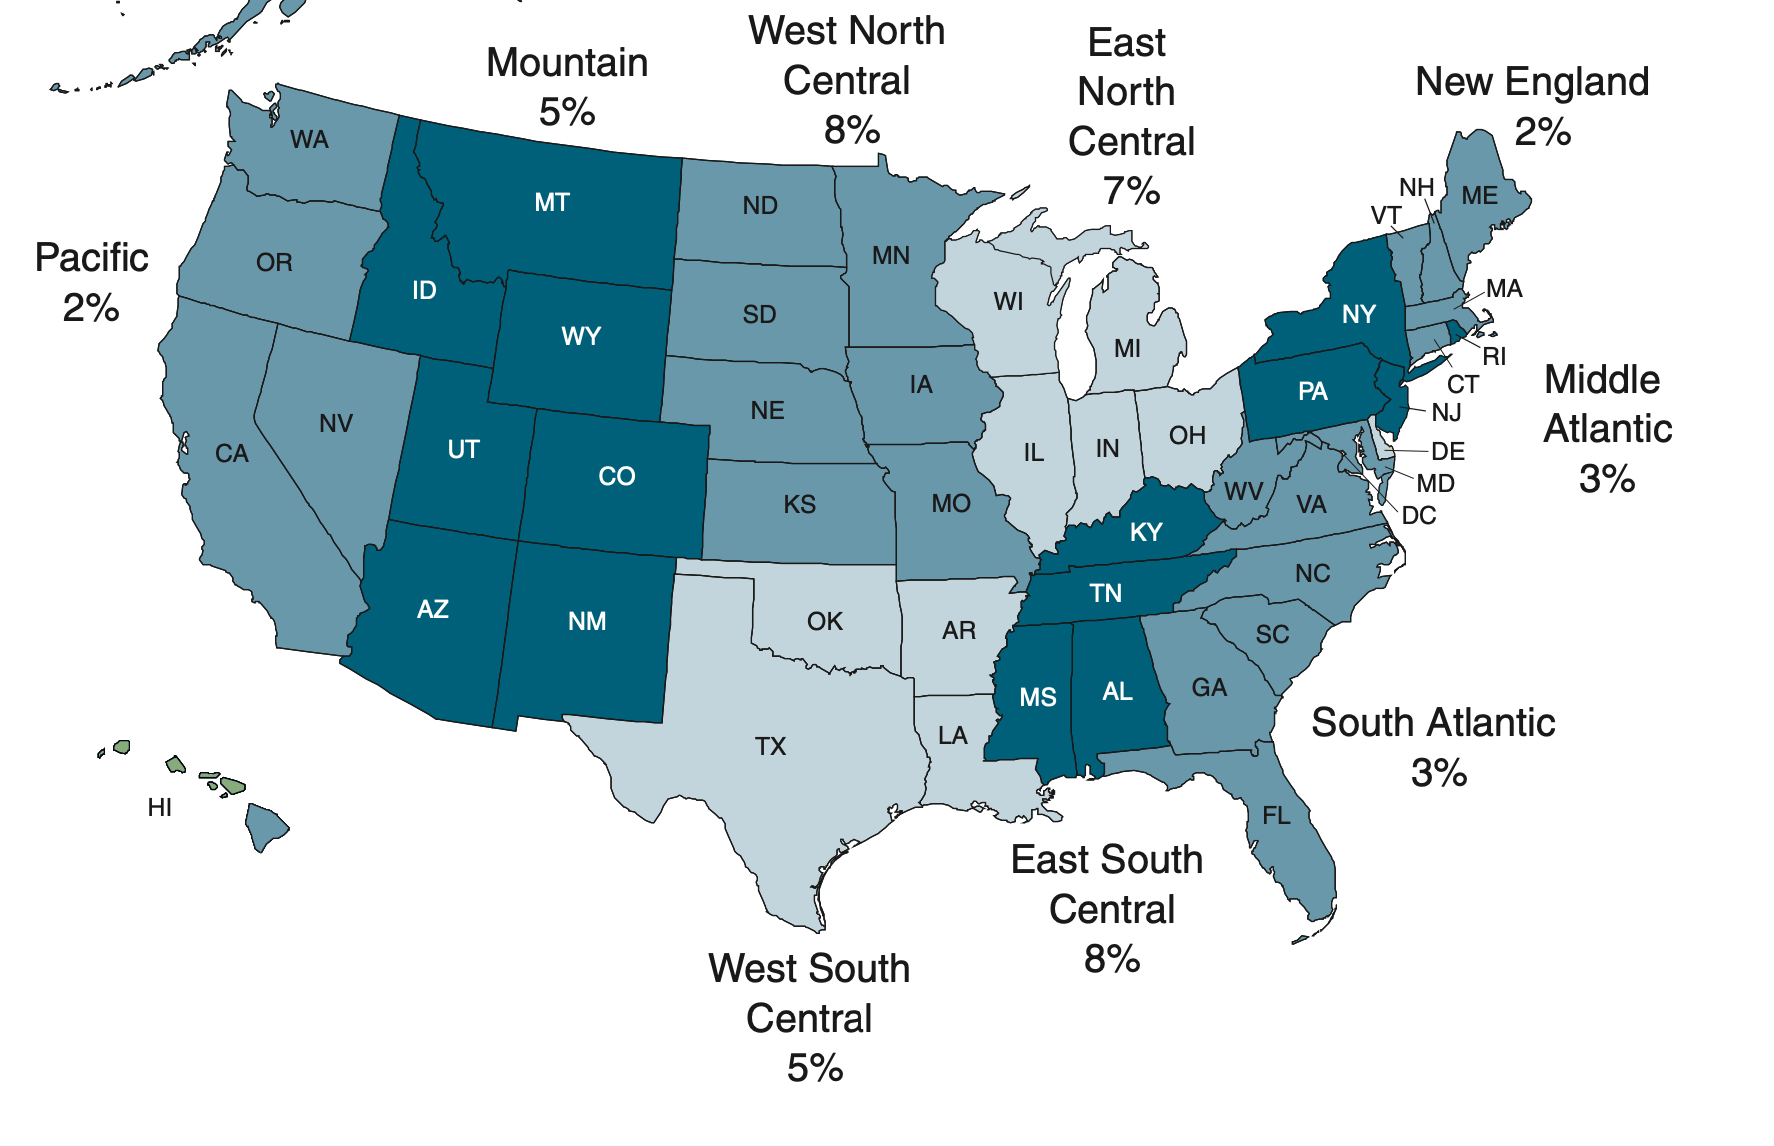
\includegraphics[width=0.75\textwidth,height=0.75\textheight]{./img/2016_fish_wildlife_report.png}
\caption{2016 National Survey of Fishing, Hunting, and
Wildlife-Associated Recreation, showing regional variation in hunting
participation rates.}\label{id}
}
\end{figure}

Various explanations for the decline in hunting have been tendered.
Researchers found evidence that more people opt for electronic
entertainment and urban living as explainations for the decline in
hunting. (Robison and Ridenour 2012)

\hypertarget{data-sources}{%
\section{Data Sources}\label{data-sources}}

Data was retrieved from two sources: the U.S. Fish and Wildlife Agency
and the U.S. Census Bureau.

\hypertarget{u.s.-fish-and-wildlife}{%
\subsection{U.S. Fish and Wildlife}\label{u.s.-fish-and-wildlife}}

States require a hunting license for those harvesting game. People who
engage in hunting within the boundaries of the state they reside in
require a ``resident'' hunting license whereas those who travel to
another state require a ``non-resident'' license. A proxy for the
popularity of the pastime is the number of hunting licenses issued by
the states. The U.S. Fish and Wildlife tracks the issuance of hunting,
and fishing, licenses.

Data is available via their
\href{https://www.fws.gov/wsfrprograms/Subpages/LicenseInfo/Hunting.htm}{website}.
Hunting license information is collected annually from (1) state, (2)
territory and (3) insular areas license certifications. The data is
available for the years 1963 - 2020 though it is in a pdf format.

\hypertarget{u.s.-census-bureau}{%
\subsection{U.S. Census Bureau}\label{u.s.-census-bureau}}

\hypertarget{methodology}{%
\section{Methodology}\label{methodology}}

The effort used a statistical programming language known as ``R''. (R
Core Team 2019)

\begin{verbatim}
## R version 3.6.3 (2020-02-29)
## Platform: x86_64-apple-darwin15.6.0 (64-bit)
## Running under: macOS Catalina 10.15.7
## 
## Matrix products: default
## BLAS:   /Library/Frameworks/R.framework/Versions/3.6/Resources/lib/libRblas.0.dylib
## LAPACK: /Library/Frameworks/R.framework/Versions/3.6/Resources/lib/libRlapack.dylib
## 
## locale:
## [1] en_US.UTF-8/en_US.UTF-8/en_US.UTF-8/C/en_US.UTF-8/en_US.UTF-8
## 
## attached base packages:
## [1] stats     graphics  grDevices utils     datasets  methods   base     
## 
## loaded via a namespace (and not attached):
##  [1] compiler_3.6.3  magrittr_1.5    tufte_0.8       formatR_1.7    
##  [5] tools_3.6.3     htmltools_0.4.0 yaml_2.2.1      Rcpp_1.0.4     
##  [9] stringi_1.4.6   rmarkdown_2.5   knitr_1.30      stringr_1.4.0  
## [13] xfun_0.18       digest_0.6.25   rlang_0.4.5     evaluate_0.14
\end{verbatim}

\begin{Shaded}
\begin{Highlighting}[]
\NormalTok{file <-}\StringTok{ "./data_tidy/hunting_licenses_by_state_2000_and_2020.csv"}
\NormalTok{df <-}\StringTok{ }\KeywordTok{read.csv}\NormalTok{(}\DataTypeTok{file =}\NormalTok{ file, }\DataTypeTok{header =}\NormalTok{ T, }\DataTypeTok{colClasses =} \StringTok{"character"}\NormalTok{)}
\KeywordTok{str}\NormalTok{(df)}
\end{Highlighting}
\end{Shaded}

\begin{verbatim}
## 'data.frame':    900 obs. of  6 variables:
##  $ fips : chr  "01" "02" "04" "05" ...
##  $ state: chr  "Alabama" "Alaska" "Arizona" "Arkansas" ...
##  $ abb  : chr  "AL" "AK" "AZ" "AR" ...
##  $ year : chr  "2000" "2000" "2000" "2000" ...
##  $ key  : chr  "certified_paid_hunting_license_holders_2000" "certified_paid_hunting_license_holders_2000" "certified_paid_hunting_license_holders_2000" "certified_paid_hunting_license_holders_2000" ...
##  $ value: chr  "271865" "97508" "196659" "395304" ...
\end{verbatim}

\begin{Shaded}
\begin{Highlighting}[]
\NormalTok{knitr}\OperatorTok{::}\KeywordTok{kable}\NormalTok{(}\KeywordTok{head}\NormalTok{(mtcars[, }\DecValTok{1}\OperatorTok{:}\DecValTok{4}\NormalTok{]), }\StringTok{"pipe"}\NormalTok{)}
\end{Highlighting}
\end{Shaded}

\begin{longtable}[]{@{}lrrrr@{}}
\toprule
& mpg & cyl & disp & hp\tabularnewline
\midrule
\endhead
Mazda RX4 & 21.0 & 6 & 160 & 110\tabularnewline
Mazda RX4 Wag & 21.0 & 6 & 160 & 110\tabularnewline
Datsun 710 & 22.8 & 4 & 108 & 93\tabularnewline
Hornet 4 Drive & 21.4 & 6 & 258 & 110\tabularnewline
Hornet Sportabout & 18.7 & 8 & 360 & 175\tabularnewline
Valiant & 18.1 & 6 & 225 & 105\tabularnewline
\bottomrule
\end{longtable}

\begin{Shaded}
\begin{Highlighting}[]
\NormalTok{knitr}\OperatorTok{::}\KeywordTok{kable}\NormalTok{(}\KeywordTok{head}\NormalTok{(mtcars[, }\DecValTok{1}\OperatorTok{:}\DecValTok{4}\NormalTok{]), }\StringTok{"simple"}\NormalTok{)}
\end{Highlighting}
\end{Shaded}

\begin{longtable}[]{@{}lrrrr@{}}
\toprule
& mpg & cyl & disp & hp\tabularnewline
\midrule
\endhead
Mazda RX4 & 21.0 & 6 & 160 & 110\tabularnewline
Mazda RX4 Wag & 21.0 & 6 & 160 & 110\tabularnewline
Datsun 710 & 22.8 & 4 & 108 & 93\tabularnewline
Hornet 4 Drive & 21.4 & 6 & 258 & 110\tabularnewline
Hornet Sportabout & 18.7 & 8 & 360 & 175\tabularnewline
Valiant & 18.1 & 6 & 225 & 105\tabularnewline
\bottomrule
\end{longtable}

\begin{Shaded}
\begin{Highlighting}[]
\NormalTok{iris2 <-}\StringTok{ }\KeywordTok{head}\NormalTok{(iris)}
\NormalTok{knitr}\OperatorTok{::}\KeywordTok{kable}\NormalTok{(iris2, }\DataTypeTok{col.names =} \KeywordTok{gsub}\NormalTok{(}\StringTok{"[.]"}\NormalTok{, }\StringTok{" "}\NormalTok{, }\KeywordTok{names}\NormalTok{(iris)))}
\end{Highlighting}
\end{Shaded}

\begin{longtable}[]{@{}rrrrl@{}}
\toprule
Sepal Length & Sepal Width & Petal Length & Petal Width &
Species\tabularnewline
\midrule
\endhead
5.1 & 3.5 & 1.4 & 0.2 & setosa\tabularnewline
4.9 & 3.0 & 1.4 & 0.2 & setosa\tabularnewline
4.7 & 3.2 & 1.3 & 0.2 & setosa\tabularnewline
4.6 & 3.1 & 1.5 & 0.2 & setosa\tabularnewline
5.0 & 3.6 & 1.4 & 0.2 & setosa\tabularnewline
5.4 & 3.9 & 1.7 & 0.4 & setosa\tabularnewline
\bottomrule
\end{longtable}

\begin{Shaded}
\begin{Highlighting}[]
\CommentTok{# left, center, center, right, right}
\NormalTok{knitr}\OperatorTok{::}\KeywordTok{kable}\NormalTok{(iris2, }\DataTypeTok{align =} \StringTok{"lccrr"}\NormalTok{, }\DataTypeTok{caption =} \StringTok{"An example of table caption"}\NormalTok{)}
\end{Highlighting}
\end{Shaded}

\begin{longtable}[]{@{}lccrr@{}}
\caption{An example of table caption}\tabularnewline
\toprule
Sepal.Length & Sepal.Width & Petal.Length & Petal.Width &
Species\tabularnewline
\midrule
\endfirsthead
\toprule
Sepal.Length & Sepal.Width & Petal.Length & Petal.Width &
Species\tabularnewline
\midrule
\endhead
5.1 & 3.5 & 1.4 & 0.2 & setosa\tabularnewline
4.9 & 3.0 & 1.4 & 0.2 & setosa\tabularnewline
4.7 & 3.2 & 1.3 & 0.2 & setosa\tabularnewline
4.6 & 3.1 & 1.5 & 0.2 & setosa\tabularnewline
5.0 & 3.6 & 1.4 & 0.2 & setosa\tabularnewline
5.4 & 3.9 & 1.7 & 0.4 & setosa\tabularnewline
\bottomrule
\end{longtable}

\begin{Shaded}
\begin{Highlighting}[]
\NormalTok{knitr}\OperatorTok{::}\KeywordTok{kable}\NormalTok{(iris2, }\DataTypeTok{caption =} \StringTok{"An example table caption."}\NormalTok{)}
\end{Highlighting}
\end{Shaded}

\begin{longtable}[]{@{}rrrrl@{}}
\caption{An example table caption.}\tabularnewline
\toprule
Sepal.Length & Sepal.Width & Petal.Length & Petal.Width &
Species\tabularnewline
\midrule
\endfirsthead
\toprule
Sepal.Length & Sepal.Width & Petal.Length & Petal.Width &
Species\tabularnewline
\midrule
\endhead
5.1 & 3.5 & 1.4 & 0.2 & setosa\tabularnewline
4.9 & 3.0 & 1.4 & 0.2 & setosa\tabularnewline
4.7 & 3.2 & 1.3 & 0.2 & setosa\tabularnewline
4.6 & 3.1 & 1.5 & 0.2 & setosa\tabularnewline
5.0 & 3.6 & 1.4 & 0.2 & setosa\tabularnewline
5.4 & 3.9 & 1.7 & 0.4 & setosa\tabularnewline
\bottomrule
\end{longtable}

\begin{Shaded}
\begin{Highlighting}[]
\KeywordTok{library}\NormalTok{(knitr)}
\KeywordTok{library}\NormalTok{(kableExtra)}
\KeywordTok{kable}\NormalTok{(iris[}\DecValTok{1}\OperatorTok{:}\DecValTok{5}\NormalTok{, ]) }\OperatorTok\StringTok{ }\KeywordTok{kable_styling}\NormalTok{(}\DataTypeTok{latex_options =} \StringTok{"striped"}\NormalTok{)}
\end{Highlighting}
\end{Shaded}

\begin{table}[H]
\centering
\begin{tabular}{r|r|r|r|l}
\hline
Sepal.Length & Sepal.Width & Petal.Length & Petal.Width & Species\\
\hline
\cellcolor{gray!6}{5.1} & \cellcolor{gray!6}{3.5} & \cellcolor{gray!6}{1.4} & \cellcolor{gray!6}{0.2} & \cellcolor{gray!6}{setosa}\\
\hline
4.9 & 3.0 & 1.4 & 0.2 & setosa\\
\hline
\cellcolor{gray!6}{4.7} & \cellcolor{gray!6}{3.2} & \cellcolor{gray!6}{1.3} & \cellcolor{gray!6}{0.2} & \cellcolor{gray!6}{setosa}\\
\hline
4.6 & 3.1 & 1.5 & 0.2 & setosa\\
\hline
\cellcolor{gray!6}{5.0} & \cellcolor{gray!6}{3.6} & \cellcolor{gray!6}{1.4} & \cellcolor{gray!6}{0.2} & \cellcolor{gray!6}{setosa}\\
\hline
\end{tabular}
\end{table}

\hypertarget{conclusions}{%
\section{Conclusions}\label{conclusions}}

Hunting license issuance among the states for the 2000 to 2020 years
declined. This conclusion is identical to other studies using the U.S.
Fish and Wildlife survey data. Possible explanations in the decline in
hunting include the aging of the U.S. population, the continued
migration from rural to urban settings. (Mehmood, Zhang, and Armstrong
2003)

\hypertarget{resources}{%
\section{Resources}\label{resources}}

\href{https://www.outdoorlife.com/why-we-are-losing-hunters-and-how-to-fix-it/}{Krebs,
Natalie, Why We Suck at Recruiting New Hunters, Why It Matters, and How
You Can Fix It, Outdoor Life (2019).}

\href{https://www.census.gov/content/dam/Census/library/publications/2018/demo/fhw16-nat.pdf}{U.S.
Department of the Interior, U.S. Fish and Wildlife Service, and U.S.
Department of Commerce, U.S. Census Bureau. 2016 National Survey of
Fishing, Hunting, and Wildlife-Associated Recreation.}

\href{https://wildlifemanagement.institute}{Wildlife Management
Institute}.

\href{https://www.fishwildlife.org}{Association of Fish and Wildlife
Agencies.}

Sayeed Mehmood, Daowei Zhang \& James Armstrong (2003) Factors
Associated with Declining Hunting License Sales in Alabama, Human
Dimensions of Wildlife, 8:4, 243-262, DOI:
\href{https://www.tandfonline.com/doi/abs/10.1080/716100423}{10.1080/716100423}

\hypertarget{bibliography}{%
\section*{Bibliography}\label{bibliography}}
\addcontentsline{toc}{section}{Bibliography}

\hypertarget{refs}{}
\leavevmode\hypertarget{ref-Mehmood}{}%
Mehmood, Sayeed, Daowei Zhang, and James Armstrong. 2003. ``Factors
Associated with Declining Hunting License Sales in Alabama.''
\emph{Human Dimensions of Wildlife} 8 (4). Routledge: 243--62.
\url{https://doi.org/10.1080/716100423}.

\leavevmode\hypertarget{ref-R-base}{}%
R Core Team. 2019. \emph{R: A Language and Environment for Statistical
Computing}. Vienna, Austria: R Foundation for Statistical Computing.
\url{https://www.R-project.org}.

\leavevmode\hypertarget{ref-Robison}{}%
Robison, Kristopher K., and Daniel Ridenour. 2012. ``Whither the Love of
Hunting? Explaining the Decline of a Major Form of Rural Recreation as a
Consequence of the Rise of Virtual Entertainment and Urbanism.''
\emph{Human Dimensions of Wildlife} 17 (6). Routledge: 418--36.
\url{https://doi.org/10.1080/10871209.2012.680174}.

\leavevmode\hypertarget{ref-rott}{}%
Rott, Nathan. 2018. ``Decline in Hunters Threatens How Us Pays for
Conservation.'' \emph{National Public Radio}.

\leavevmode\hypertarget{ref-winkler}{}%
Winkler, Richelle, and Keith Warnke. 2013. ``The Future of Hunting: An
Age-Period-Cohort Analysis of Deer Hunter Decline.'' \emph{Population
and Environment} 34 (4). Springer: 460--80.
\url{https://doi.org/10.1007/s11111-012-0172-6}.



\end{document}
